\chapter{Historia i rozwój robotyki}
\label{ch:history}
Robotyka jest stosunkowo młodą dziedziną łączącą różne gałęzie nauk technicznych
i nie tylko. Do pełnego zrozumienia zagadnień współczesnej robotyki oraz budowy
i~zastosowań robotów konieczna jest niejednokrotnie rozległa wiedza na temat
elektroniki, mechaniki, inżynierii przemysłowej, matematyki oraz szeroko pojętej
informatyki. Ponadto wiele nowopowstałych gałęzi wiedzy zajmujących się rozwojem
sztucznej inteligencji, modelowaniem sztucznego życia czy rozwojem inżynierii
wiedzy coraz częściej staje się nierozerwalnie związane z problemami współczesnej
robotyki. Nie~należy zapominać również o tym, że rozwój inżynierii wytwarzania
oraz automatyki przemysłowej pozwala na~nieustanny rozwój robotyki z którą mamy
do czynienia w przemyśle w dniu dzisiejszym.

\section{Historia robotyki}
Pojęcie ,,robot'' w literaturze pojawiło się po raz pierwszy w sztuce czeskiego
pisarza Karel'a Capka w roku 1920. Termin ,,robot'' oznacza w języku czeskim
pracę lub służbę przymusową. Nieco ponad 20 lat później, amerykański uczony i
pisarz Isaac Assimov w~jednym ze swoich opowiadań po raz pierwszy używa słowa
robotyka. W kolejnych latach Assimov w swojej twórczości niejednokrotnie wraca do
problemu robotyki skutkiem czego jest wydanie w 1950 roku zbioru opowiadań pod
tytułem ,,Ja, robot''. Jako ciekawostkę można dodać, że w wydanym w 1942 roku
opowiadaniu pod tytułem ,,Zabawa w berka'', Assimov wprowadza trzy prawa robotyki
według których, zdaniem autora, powinny być programowane roboty\cite{Runaround}.
Zdefiniowane przez Assimov'a prawa robotyki w pełnym brzmieniu widoczne są na
diagramie \ref{fig:Assimov_Laws}.
% \begin{description}
% \item[Prawo pierwsze] \hfill \\
% Robot nie może zranić istoty ludzkiej, ani przez zaniedbanie narazić człowieka
% na zranienie.
% \item[Prawo drugie] \hfill \\
% Robot musi spełniać polecenia wydawane przez człowieka, poza poleceniami
% sprzecznymi z prawem pierwszym.
% \item[Prawo trzecie] \hfill \\
% Robot musi chronić samego siebie dopóki nie jest to sprzeczne z prawami
% pierwszym i drugim. \end{description}

\begin{figure}[h!] \centering
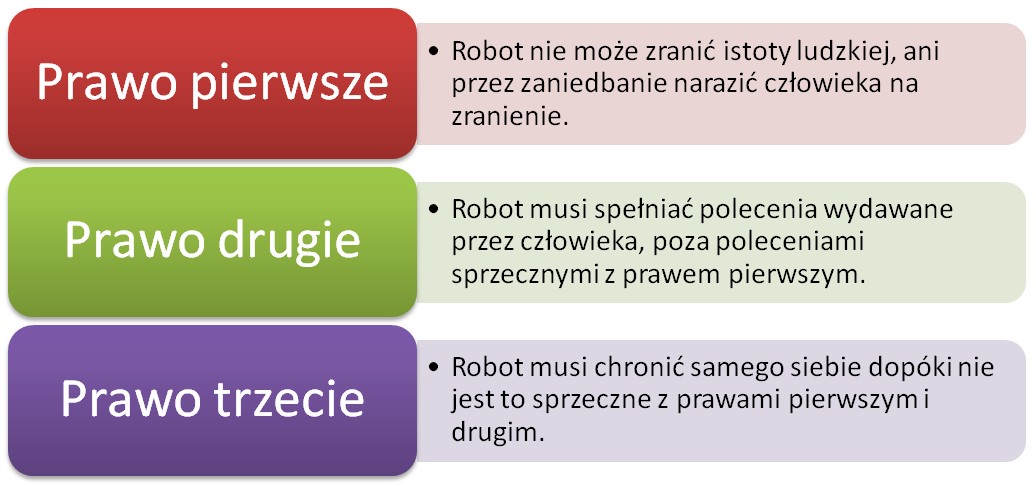
\includegraphics[height=70mm]{../images/ch01/assimov_laws.png}
	\caption{Prawa robotyki zdefiniowane przez Issaca Assimov'a}
	\label{fig:Assimov_Laws}
\end{figure}

Nieco później, Isaac Assimov, jako uzupełnienie i prawo nadrzędne dodaje prawo
zerowe o następującym brzmieniu ,,Robot nie może szkodzić ludzkości, ani przez
zaniedbanie narazić ludzkości na szkodę''\cite{website:robotyka-pl}. Oprócz
wspomnianych powyżej podstawowych praw, zdefiniowano również inne prawa
wynikające z prowadzonych w tej dziedzinie badań i~rozwoju robotyki. \newpage
Takim sposobem urządzenie mechaniczne wykonujące zadania w sposób automatyczny
otrzymało miano ,,robota''\cite{website:asimo-pl}. Operacje wykonywane przez
robota mogą być bezpośrednio kontrolowane przez człowieka na podstawie
przygotowanego wcześniej programu zawierającego zestaw reguł które umożliwiają
robotowi wykonywanie określonych czynności. Możliwość wyręczenia człowieka przez
maszynę w wykonywaniu monotonnych, złożonych i powtarzalnych czynności,
niejednoktornie z dużo większą wydajnością i precyzją, była jednym z podstawowych
bodźców który sprzyjał rozwojowi robotyki już od samego jej początku. Pojęcie
robot, używane jest również w stosunku do autonomicznie działających urządzeń
pobierających informację z~otocznia za pomocą różnego rodzaju czujników,
nazywanych sensorami, oraz oddziałujących na swoje otoczenie i reagujące na jego
zmiany.

Dzięki gwałtownemu rozwojowi nauki i techniki w czasie II wojny światowej w roku
1956 GC.~Devol i JF. Engelberger zainspirowani twórczością Assimov'a
zaprojektowali i~stworzyli pierwszy w dziejach ludzkości działający egzemplarz
robota\cite{website:robotyka-pl}. Engelberger założył firmę pod nazwą
,,Unimation'' zajmującą się automatyzacją, pierwszym robotem stworzonym przez
firmę Engelbergera był robot nazwany ,,Unimate''. Został on zainstalowany w
fabryce General Motors w Trenton gdzie został przystosowany do obsługi
wysokociśnieniowej maszyny odlewniczej. W~kolejnych latach roboty firmy
,,Unimation'' znalazły swoje zastosowanie w~innych gałęziach przemysłu, a sam
Engelberger otrzymał miano ojca robotyki.\cite{website:robotyka-pl}
 
Nieco później, bo w roku 1979 Robotics Industries Association zdefiniowało robota
jako wielofunkcyjny, programowalny manipulator zaprojektowany do przenoszenia
materiałów, narzędzi, części urządzeń poprzez serię programowalnych ruchów
wykonywanych w celu realizacji różnych zadań. W myśl wspomnianej definicji jedną
z podstawowych cech robota jest jego programowalność i możliwość dostosowywania
się do zmiennych warunków środowiska pracy.

Pierwsze roboty projektowano z myślą o zastosowaniu ich do realizacji
elementarnych zadań związanych z przenoszeniem elementów z jednego punktu do
drugiego. Program pracy robota miał więc charakter sekwencji operacji
prowadzących do realizacji określonego przez programistę zadania. W miarę rozwoju
technicznego, stawiane przed robotami zadania wymusiły użycie przez konstruktorów
czujników które pozwalały na~zwiększenie poziomu interakcji robotów z otoczeniem,
a co za tym idzie umożliwiły realizowanie zadań o wysokim stopniu złożoności. Od
tego momentu kierunek rozwoju robotyki obrał sobie za cel stworzenie maszyny na
tyle uniwersalnej i niezależnej aby mogła nosić miano androida. Jednak do
realizacji tego zadania konieczne jest opracowanie sztucznej inteligencji na
którą z pewnością przyjdzie nam jeszcze trochę poczekać.

Pierwszym krokiem na drodze do stworzenia androida było oderwanie robota
od~stałego miejsca instalacji i pozwolenie mu w miarę możliwości swobodne
poruszanie się w~dostępnej mu przestrzeni roboczej. Tak powstała klasa robotów
które mogą przemieszczać się za pomocą kół, gąsienic czy nawet kończyn lub
odnóży. Roboty tego typu potrafią pływać, latać i sprawnie poruszać się po lądzie
dodatkowym ich atutem jest fakt iż większość z nich posiada niemal całkowitą
autonomię i ograniczona jest jedynie poprzez wielkość otoczenia w jakim zostały
umieszczone. Takim sposobem powstała grupa robotów nazywanych robotami mobilnymi.
Cechą wspólną wszystkich urządzeń z~tej rodziny była umiejętność swobodnego
przemieszczania się oraz analiza najbliższego otoczenia. Na~tej podstawie maszyna
mogła przeprowadzić wnioskowanie pozwalające na~podejmowanie dalszych akcji czy
też przesłanie użytkownikowi odczytanych parametrów środowiska.

Historię robotów mobilnych zapoczątkował amerykański Uniwersytet w Stanford gdyż
w roku 1968 jako pierwszy stworzył w pełni działający model robota mobilnego pod
nazwą Shakey (rys. \ref{fig:RobotsHistory_Shakey_Genghis}). Nazwa została
zainspirowana szarpanymi ruchami z jakimi robot się poruszał. Głównym zadaniem
robota było modelowanie otoczenia w którym się znajdował. W ślad za Uniwersytetem
w Stanford ruszyło MIT. W roku 1983 posiadali już pierwszy działający model
robota swobodnie skaczącego. Niecałe 6 lat później MIT stworzyło pierwszego
robota kroczącego wzorowanego na owadach. Robot ten sterowany był za pomocą
wielowarstwowych automatów o stanach skończonych, a ze światem zewnętrznym
komunikował się za pomocą czułek, inklinometrów, czujników zbliżeniowych na
podczerwień. Genghis, bo tak nazwany został robot, posiadał na pokładzie 4
ośmiobitowe jednostki obliczeniowe, ważył niecały kilogram i miał 35 cm długości.

\begin{figure}[h!]
 \centering
 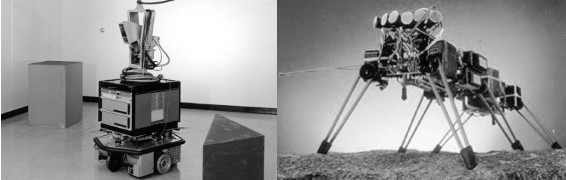
\includegraphics[width=\textwidth]{../images/ch01/shakey_and_genghis.png}
 \caption{Pierwsze roboty. Od lewej: Shakey (Stanford), Genghis (MIT) }
 \label{fig:RobotsHistory_Shakey_Genghis}
\end{figure}

Po sukcesie wspomnianych projektów, rozwój robotów mobilnych następował już
bardzo dynamiczne. W latach 90 powstawało wiele różnych modeli robotów o bardzo
różnorodnych rodzajach napędów oraz zestawach czujników umożliwiających
interakcje ze światem zewnętrznym.

Swoistym ukoronowaniem prac było w 1997 roku stworzenie przez NASA robota
o~nazwie Pathfinder. Robot wyposażony był w czujniki laserowe, stereowizję,
żyroskopy i~inne rodzaje czujników o charakterze badawczym. Zasilany był on
bateriami słonecznymi które pozwoliły mu na 83 dni nieprzerwanej pracy podczas
której robot przebył około 100 metrów i wykonał 230 manewrów. W ostatnich latach
do największych osiągnięć robotyki mobilnej można z pewnością zaliczyć powstanie
robotów humanoidalnych takich jak japoński ASIMO (rys.
\ref{fig:RobotsHistory_Pathfinder_Asimo}).

\begin{figure}[h!]
 \centering
 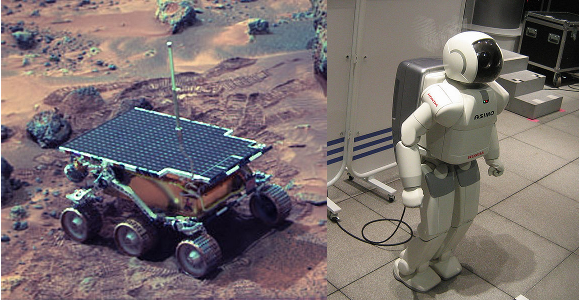
\includegraphics[height=75mm]{../images/ch01/pathfinder_and_asimo.png}
 \caption{Współczesne roboty. Kolejno: Pathfinder (NASA), Asimo (Honda)}
 \label{fig:RobotsHistory_Pathfinder_Asimo}
\end{figure}

Robot ten ważył 54 kg i posiadał 130 cm wysokości. Wersja z roku 2005 potrafiła
biegnąc osiągnąć prędkość dochodzącą nawet do do 6 km/h. Ponadto robot potrafił
wchodzić w interakcję z otaczającymi go ludźmi i przedmiotami. Urządzenie
stworzone przez inżynierów z firmy Honda potrafiło rozpoznawać gesty takie jak
podanie ręki, wskazanie kierunku czy machanie ręką na pożegnanie. Robot równie
dobrze radził sobie z rozpoznawaniem twarzy, dźwięków i analizą otaczającego go
środowiska. Potrafił on rozpoznać i~omijać niebezpieczeństwa postawione na jego
drodze jak na przykład schody czy osoby poruszające się w jego kierunku.

W roku 2006 podczas Robot World w Seulu grupa południowokoreańskich inżynierów
prezentuje swojego robota EveR-2. EveR są robotami posiadającymi wygląd typowej
dwudziestoletniej koreanki. Urządzenie potrafi rozmawiać i śpiewać dzięki
wbudowanemu ,,silnikowi dialogu'' (ang. embedded dialogue engine). Android EveR-2
w odróżnieniu od~swojej poprzedniczki ma udoskonalony system wizyjny oraz
możliwość wyrażania emocji takich jak znudzenie, zadowolenie, żal czy radość.
Robot ma 170 cm wzrostu i waży około 60 kg. Twarz androida posiada wysoką
elastyczność i poruszana jest przy pomocy 29 silniczków i licznych stawów które
pozwalają na pełną swobodę w wyrażaniu emocji. Wbudowany system rozpoznawania i
syntezy mowy w połączeniu z możliwością wyrażania się za pomocą gestów pozwala na
niemal całkowitą swobodę podczas rozmowy z~robotem. Możliwości komunikacyjne
robota są tak znakomite, że EveR-2 została pierwszą piosenkarką androidem. Jej
pierwszy występ odbył się podczas jej prezentacji w Seulu gdzie na~oczach
publiczności odśpiewała koreańską balladę pt. ,,I will close my eyes for you''.

Lata 2008 i 2009 zaowocowały powstaniem wielu robotów naśladujących w swoim
zachowaniu niektóre zwierzęta. Bardzo imponującym przykładem takiego robota jest
wyprodukowany przez firmę AeroVironment latający robot o nazwie Mercury.
Urządzenie to potrafi ,,zawisnąć'' w powietrzu poruszając jedynie skrzydłami
dokładnie w taki sam sposób jak robią to prawdziwe kolibry. Lata te były również
obfite w sukcesy w dziedzinie rozwoju sztucznego mózgu i sztucznej inteligencji.
W roku 2008 grupa naukowców z University of Reading zbudowała robota sterowanego
w całości za pomocą biologicznego mózgu z wyhodowanych neuronów. Biologiczny mózg
w który wyposażony został zainstalowany w macierzy wieloelektrodowej (MEA). MEA
jest to pewnego rodzaju naczynie które za pomocą około 60 elektrod przechwytuje
sygnały elektryczne generowane przez komórki nerwowe i przekłada je na ruchy
robota. W przypadku gdy~robot napotka na swojej drodze przeszkody wspomniane
wcześniej elektrody stymulują komórki nerwowe które tą samą drogą udzielają
instrukcji na zachowania kół które pozwoliłoby na ominięcie wykrytej przeszkody.
Robot jest
całkowicie samodzielny i~w~całości sterowany przez własny mózg.\\
\\
Obserwując postęp w dziedzinie robotyki można odnieść wrażenie iż w dzisiejszych
czasach roboty znalazły dla siebie zastosowanie niemal w każdej dziedzinie życia.
Od~wielu lat sprawdzają się już w przemyśle, transporcie, budownictwie oraz
są~niezastąpione w środowiskach nieprzyjaznych człowiekowi, takich jak podmorskie
głębiny czy otchłań kosmosu. Obszar zastosowań robotów jest tak szeroki iż
wydawać się może, że~jedynym czynnikiem ograniczającym rozwój współczesnej
robotyki są względy czysto technologiczne. Nie staje to jednak na przeszkodzie do
projektowania i tworzenia przez konstruktorów z całego świata rozwiązań coraz
bardziej przybliżających ludzkość do~stworzenia w pełni samodzielnego oraz
inteligentnego androida.
\section{Obecny rozwój i zakres zastosowań robotyki}
Robotyka zawładnęła wieloma dziedzinami życia człowieka od przemysłu poprzez
zastosowania medyczne, wojskowe aż po urządzenia stosowane w gospodarstwach
domowych. Roboty znalazły dla siebie zastosowanie w wykonywaniu zadań
wymagających dużej szybkości, dokładności i wytrzymałości której nie może
zapewnić praca wykonywana przez ludzi. W rezultacie wiele zadań wykonywanych w
produkcyjnych zakładach pracy, dawniej wykonywane przez ludzi, zostało zastąpione
przez roboty. Efektem tego jest zmniejszenie kosztów produkcji towarów masowych,
szczególnie widocznych w przypadku części samochodowych i elektroniki.
Zastosowanie robotów powoduje więc wzrost efektywności ekonomicznej i skraca czas
uruchomienia produkcji, a co za tym idzie jest głównym czynnikiem ekonomicznym
wspomagającym rozwój robotyki.

Istnieje szereg zadań które człowiek wykonuje lepiej niż maszyna, ale ze względu
na~męczący charakter pracy lub niebezpieczne środowisko jej wykonywania praca
ludzka jest zastępowana przez maszyny. Stały rozwój technologii stosowanych w
robotyce skutkuje w powstawaniu coraz bardziej zaawansowanych systemów co sprzyja
powszechniejszemu ich stosowaniu. Zastosowanie robotów w życiu codziennym
prowadzi do zwiększenia bezpieczeństwa pracy szczególnie na stanowiskach pracy
zagrażających zdrowiu i życiu człowieka. Co więcej stały rozwój robotyki pozwala
na prowadzenie badań w lokalizacjach fizycznie niedostępnych dla człowieka.
Bardzo dobrym tego przykładem jest eksploracja odległych planet czy też wnętrz
wulkanów. Jak można więc zauważyć rozwój robotyki stał się w chwili obecnej
samonapędzającą się maszyną, w której powstawanie coraz doskonalszych robotów
zwiększa na nie zapotrzebowanie, a to z kolei wymusza dalszy ich~rozwój.
\newpage\section{Klasyfikacja robotów} Współczesna różnorodność robotów
doprowadziła do powstania wielu podziałów robotów ze względu na szereg różnych
parametrów. Jednym z bardzo często spotykanych podziałów jest klasyfikacja ze
względy na sposób programowania i możliwości komunikacyjne. Każda z grup tworzy
tzw. generacje robotów. Można wyróżnić trzy generacje robotów (rys.
\ref{fig:RobotsGenerations}) uwzględniając różnice w ich układzie sterowania oraz
dostępne sensory\cite{website:robotyka-pl}.
% \begin{description} \item[Roboty I generacji] to urządzenia zaprogramowane do
% wykonywania określonej sekwencji czynności z możliwością ich przeprogramowania.
% W robotach tej generacji stosuje się otwarty układ sterowania który
% charakteryzuje się całkowitym brakiem możliwości pobierania informacji ze
% świata zewnętrznego. Do robotów pierwszej generacji zaliczyć można roboty
% przemysłowe przeznaczone do podawania i odbierania obiektów z linii
% produkcyjnej. \item[Roboty II generacji] to maszyny wyposażone w zamknięty
% układ sterowania. Oznacza to, że posiadają one zestaw czujników umożliwiających
% dokonywanie pomiarów stanu robota oraz jego otoczenia. Pozwala to robotowi na
% rozpoznanie żądanego obiektu nawet wówczas, gdy przemieszcza się wśród innych
% obiektów. Robot tej generacji powinien być w stanie podjąć decyzję na temat
% sposobu realizacji zadania na podstawie aktualnego stanu otoczenia i obiektu
% manipulacji. \item[Roboty III generacji] to urządzenia również wyposażone w
% zamknięty układ sterowania oraz zestaw czujników umożliwiających dokonywanie
% skomplikowanych pomiarów i klasyfikację obiektów o wysokim stopniu złożoności.
% System sterowania robota tej generacji powinien pozwalać na jego adaptację w
% nieznanym otoczeniu. \end{description}
\begin{figure}[h!]
 \centering 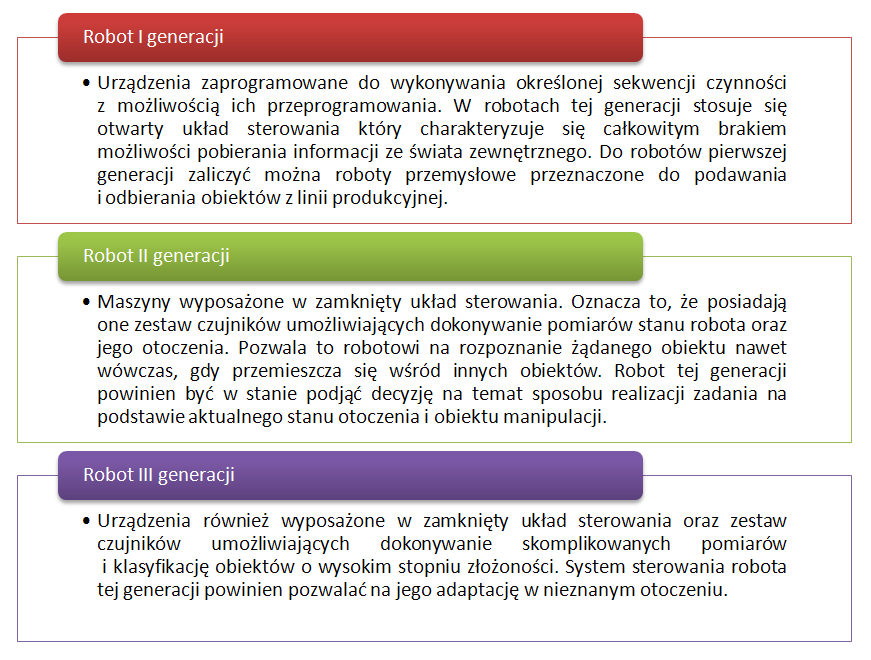
\includegraphics[height=120mm]{../images/ch01/robot_generations.png}
 \caption{Klasyfikacja robotów ze względu na ich generację}
 \label{fig:RobotsGenerations}
\end{figure}

Istnieje szereg różnych klasyfikacji robotów bazujących na podziale ze względu na
ich parametry techniczne. Jednym z bardziej znanych podziałów jest przedstawiona
poniżej klasyfikacja ze względu na rodzaj środowiska w sposób w jaki się
poruszają.
\begin{itemize}
  \item roboty podwodne i poruszające się na wodzie,
  \item roboty lądowe oraz wodno-lądowe
  \item roboty powietrzne,
\end{itemize}

Wśród robotów lądowych bardzo popularną grupą są roboty mobilne, podział których
można przeprowadzić na podstawie sposobie poruszania się. Za pomocą takiego
kryterium możemy wyróżnić roboty kołowe, kroczące, skaczące oraz pełzające.
Innym popularnym sposobem klasyfikacji robotów jest podział ze względu na 
obszar ich zastosowania. Stosując kryterium takiego rodzaju istnieje możliwość
wyróżnienia grup przedstawionych na rysunku \ref{fig:RobotsDiv}
% \begin{itemize}
%   \item roboty przemysłowe,
%   \item roboty badawczo-rozwojowe, eksploracyjne, poszukiwacze, kosmiczne,
%   \item roboty wojskowe i policyjne,
%   \item roboty do gospodarstwa domowego,
%   \item roboty usługowe sektora publicznego (społeczne, interaktywne i
%   terapeutyczne),
%   \item roboty medyczne i egzoszkielety,
% \end{itemize}
\begin{figure}[hb]
 \centering
 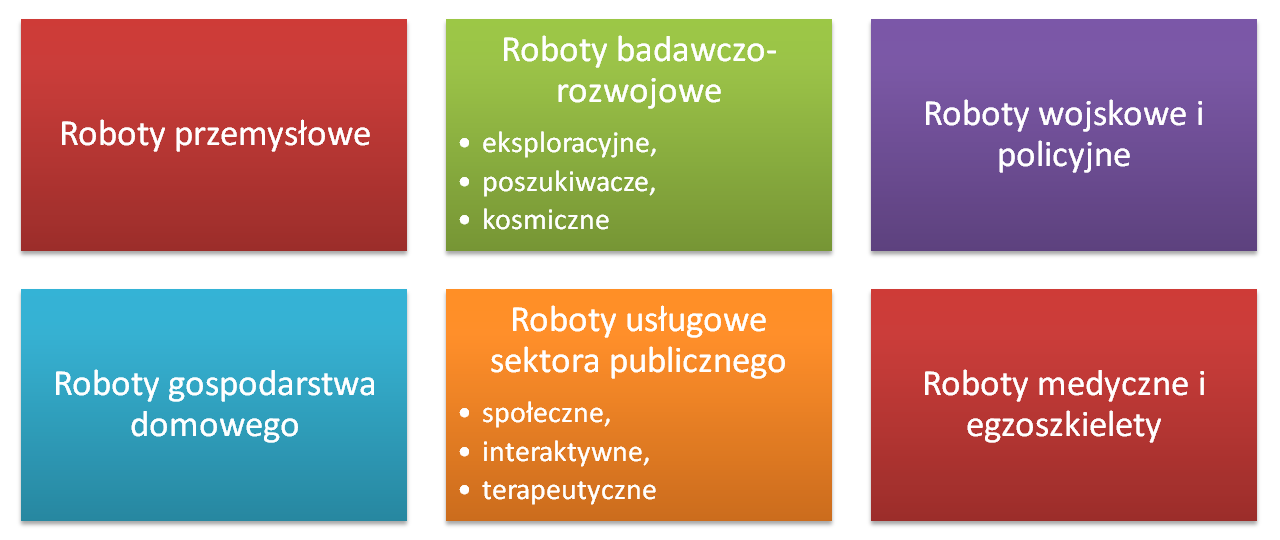
\includegraphics[width=\textwidth]{../images/ch01/robot_types.png}
 \caption{Podział robotów ze względu na obszar ich zastosowania}
 \label{fig:RobotsDiv}
\end{figure}

Omówione sposoby klasyfikacji nie wyczerpują w pełni problemu podziału
robotów i ich zastosowań. Istnieje bowiem wiele charakterystyk opartych o takie
parametry jak~na~przykład kształt czy rodzaj układu napędowego o których w tym
rozdziale nie~wspomniano. Celem przedstawionych informacji było zakreślenie
obszaru zastosowań robotów oraz bogactwa ich różnorodności, a co za tym idzie
uświadomienie czytelnikowi obszarów zastosowań robotyki we współczesnym świecie
jak również potencjalnych problemów z~jakim na codzień zmagają się ludzie
projektujący i budujący roboty.